% SBB Beamer Präsentation: Kurzfassung
\documentclass{beamer}

% Sprache und Encodings
\usepackage[ngerman]{babel}
\usepackage[utf8]{inputenc}
\usepackage[T1]{fontenc}

% Schrift: serifenlos
\usepackage{helvet}
\renewcommand{\familydefault}{\sfdefault}

% Farben (SBB-Design)
\usepackage{xcolor}
\definecolor{sbbred}{HTML}{E2001A}
\definecolor{sbbgray}{HTML}{4D4D4D}

% Beamer Theme und Farben
\usetheme{Madrid}
\usecolortheme[named=sbbred]{structure}
\setbeamercolor{title}{fg=white,bg=sbbred}
\setbeamercolor{frametitle}{fg=white,bg=sbbred}
\setbeamercolor{section in head/foot}{bg=sbbred,fg=white}
\setbeamercolor{subsection in head/foot}{bg=sbbgray,fg=white}
\setbeamercolor{footer}{fg=white}
\setbeamertemplate{footline}{%
  \leavevmode%
  \hbox{%
    \begin{beamercolorbox}[wd=1\paperwidth,ht=2.5ex,dp=1.125ex]{footer}%
      \hspace{1em}\insertshortauthor\hfill\insertframenumber{}/\inserttotalframenumber\hspace{1em}%
    \end{beamercolorbox}%
  }%
  \vskip0pt%
}

% Tabellen und Grafiken
\usepackage{graphicx}
\usepackage{booktabs}
\usepackage{float}
\usepackage{pgfplots}
\pgfplotsset{compat=1.18}

% ----- Metadaten -----
\title{Optimierte Schwellwertsetzung}
\subtitle{Kurzfassung mit den wichtigsten Ergebnissen}
\author{Carina Santos}
\date{\today}
\titlegraphic{
\includegraphics[height=1cm]{images/sbb_logo.png}}

\begin{document}

\begin{frame}[plain]
  \titlepage
\end{frame}

\begin{frame}{Monatswerte Januar (Uebersicht)}
  \textbf{Kennzahlen 2017--2026}
  \vspace{0.3cm}
  \begin{table}[H]
    \centering
    \begin{tabular}{lrrrr}
      \toprule
      Jahr & Mittelwert & Varianz & p95 & p99 \\
      \midrule
      2017 & 328.32 & 10378.15 & 491.84 & 550.24 \\
      2018 & 284.75 & 8889.74 & 437.26 & 491.29 \\
      2019 & 311.24 & 10115.45 & 474.97 & 532.80 \\
      2020 & 294.85 & 9293.84 & 453.35 & 512.55 \\
      2026 & 307.29 & 10329.21 & 471.64 & 531.97 \\
      \bottomrule
    \end{tabular}
  \end{table}
  \vspace{0.3cm}
  {\small \textbf{Insights:} Stabiles Niveau mit Ausreissern in 2017 und 2019}
\end{frame}

\begin{frame}[fragile]{Januar -- Mittelwerte}
  \begin{center}
    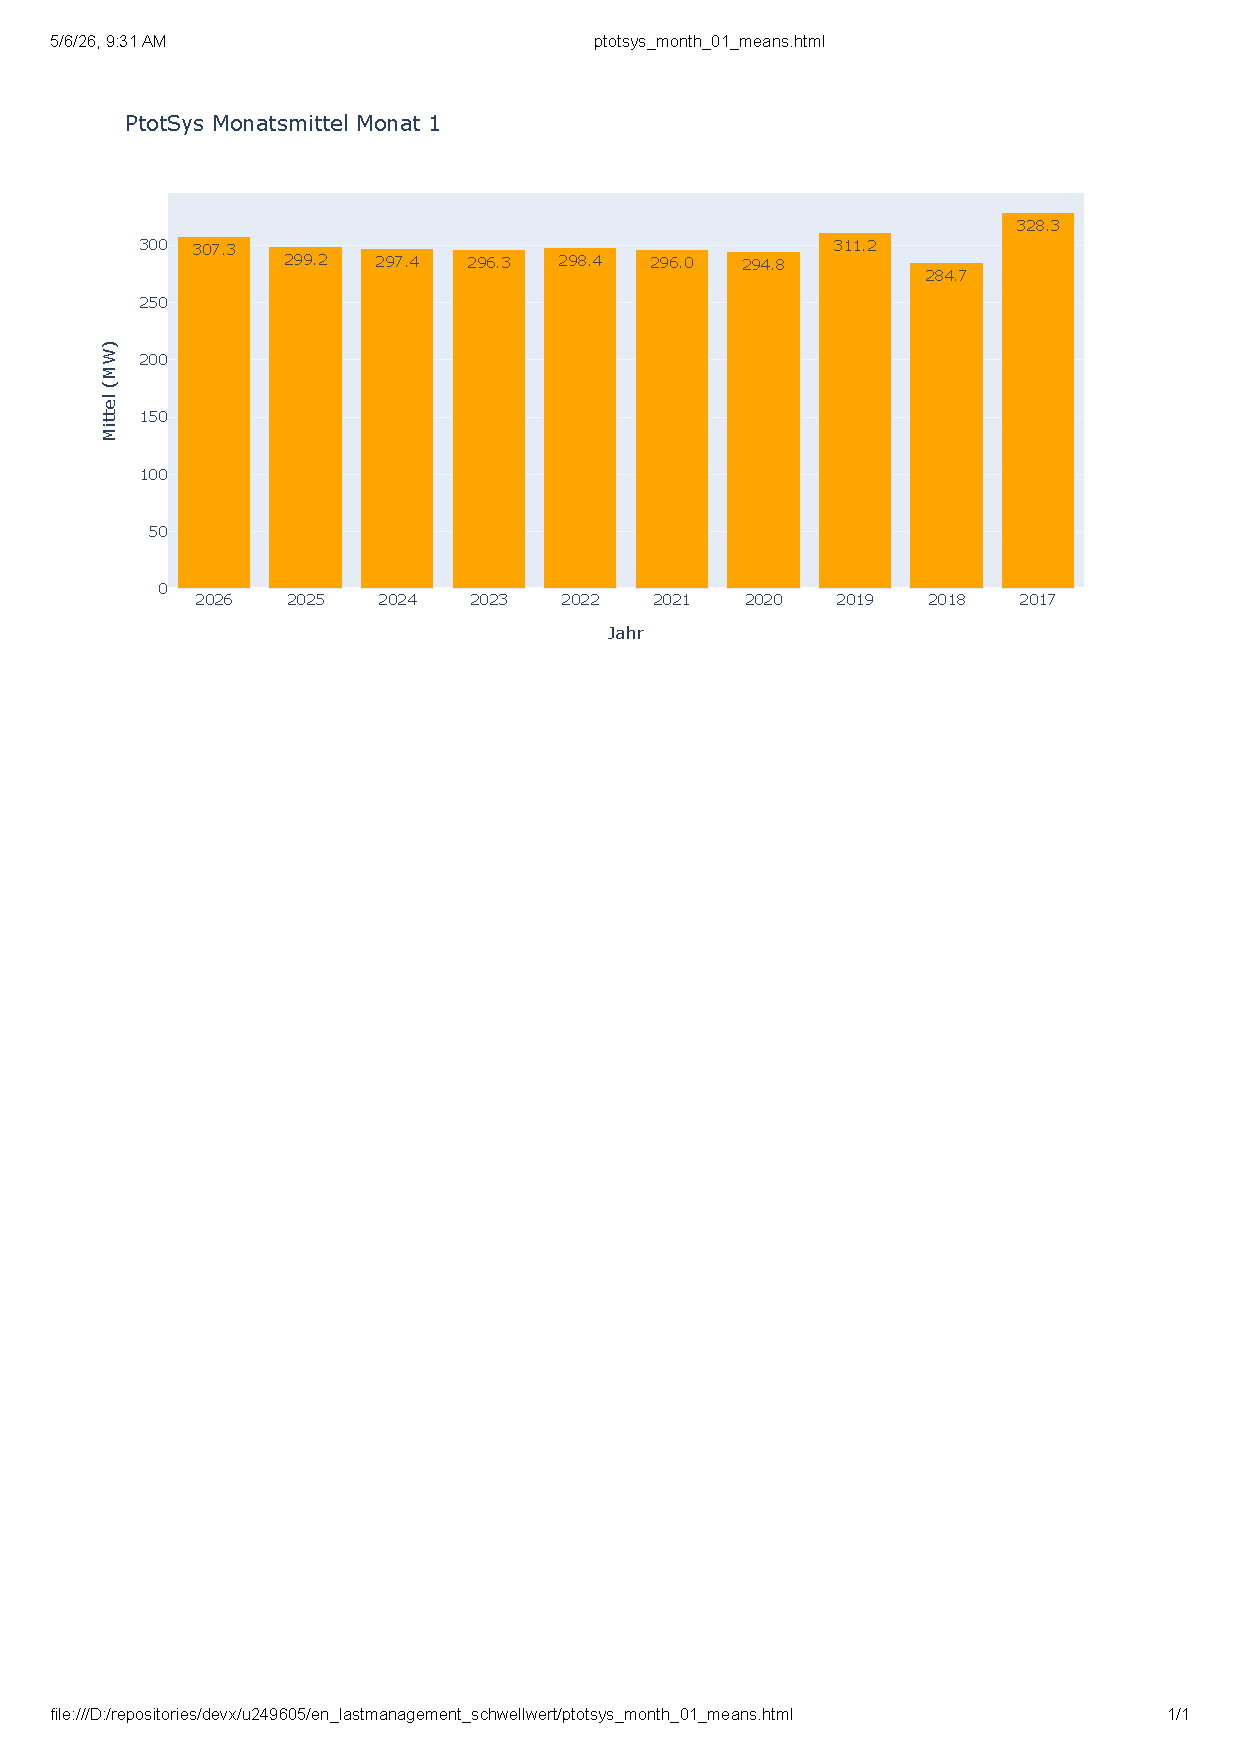
\includegraphics[width=0.95\textwidth,trim={1.2cm 18.9cm 1.2cm 3.1cm},clip]{images/ptotsys_month_01_means.html.pdf}
  \end{center}
\end{frame}

\begin{frame}[fragile]{Januar -- Varianz}
  \begin{center}
    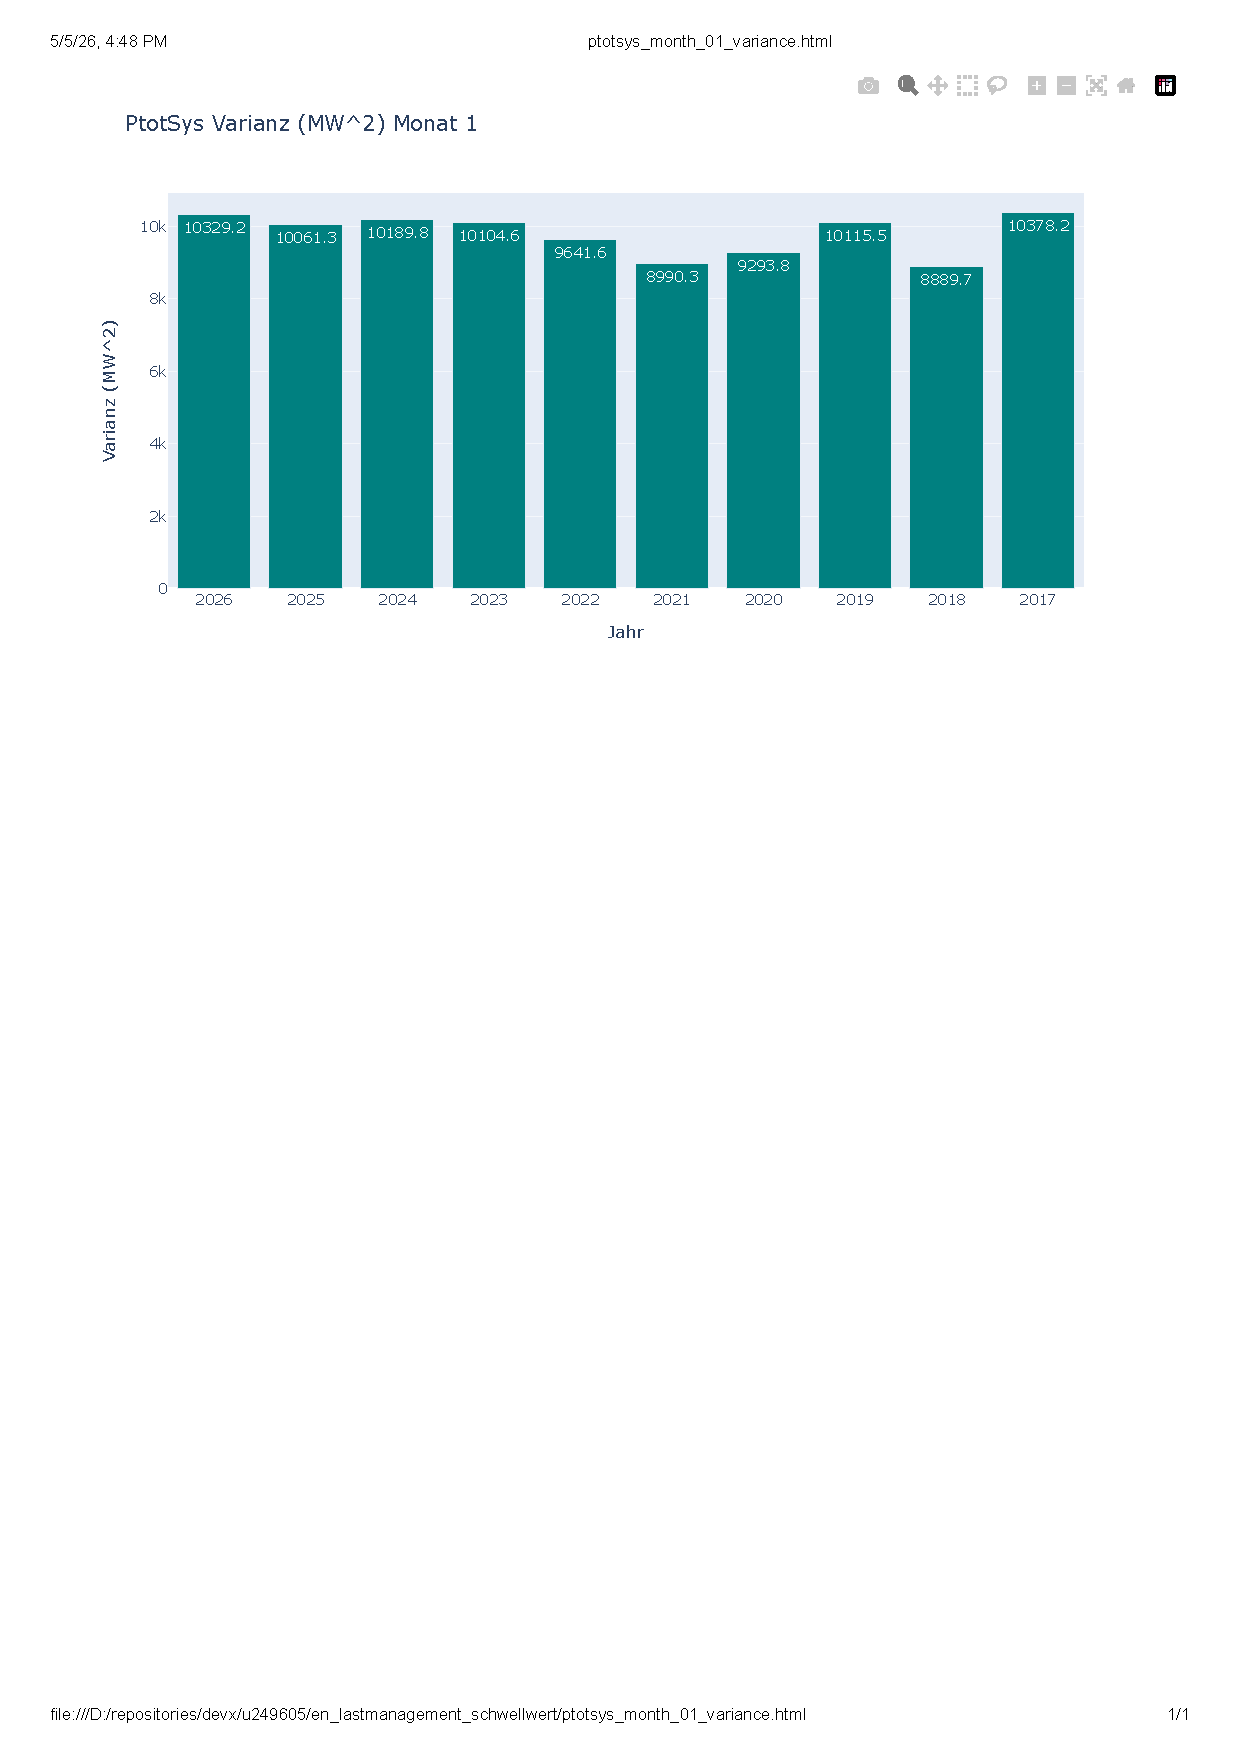
\includegraphics[width=0.95\textwidth,trim={1.2cm 18.6cm 1.2cm 3.1cm},clip]{images/ptotsys_month_01_variance.html.pdf}
  \end{center}
\end{frame}

\begin{frame}[fragile]{Januar -- Perzentile (p95 und p99)}
  \begin{center}
    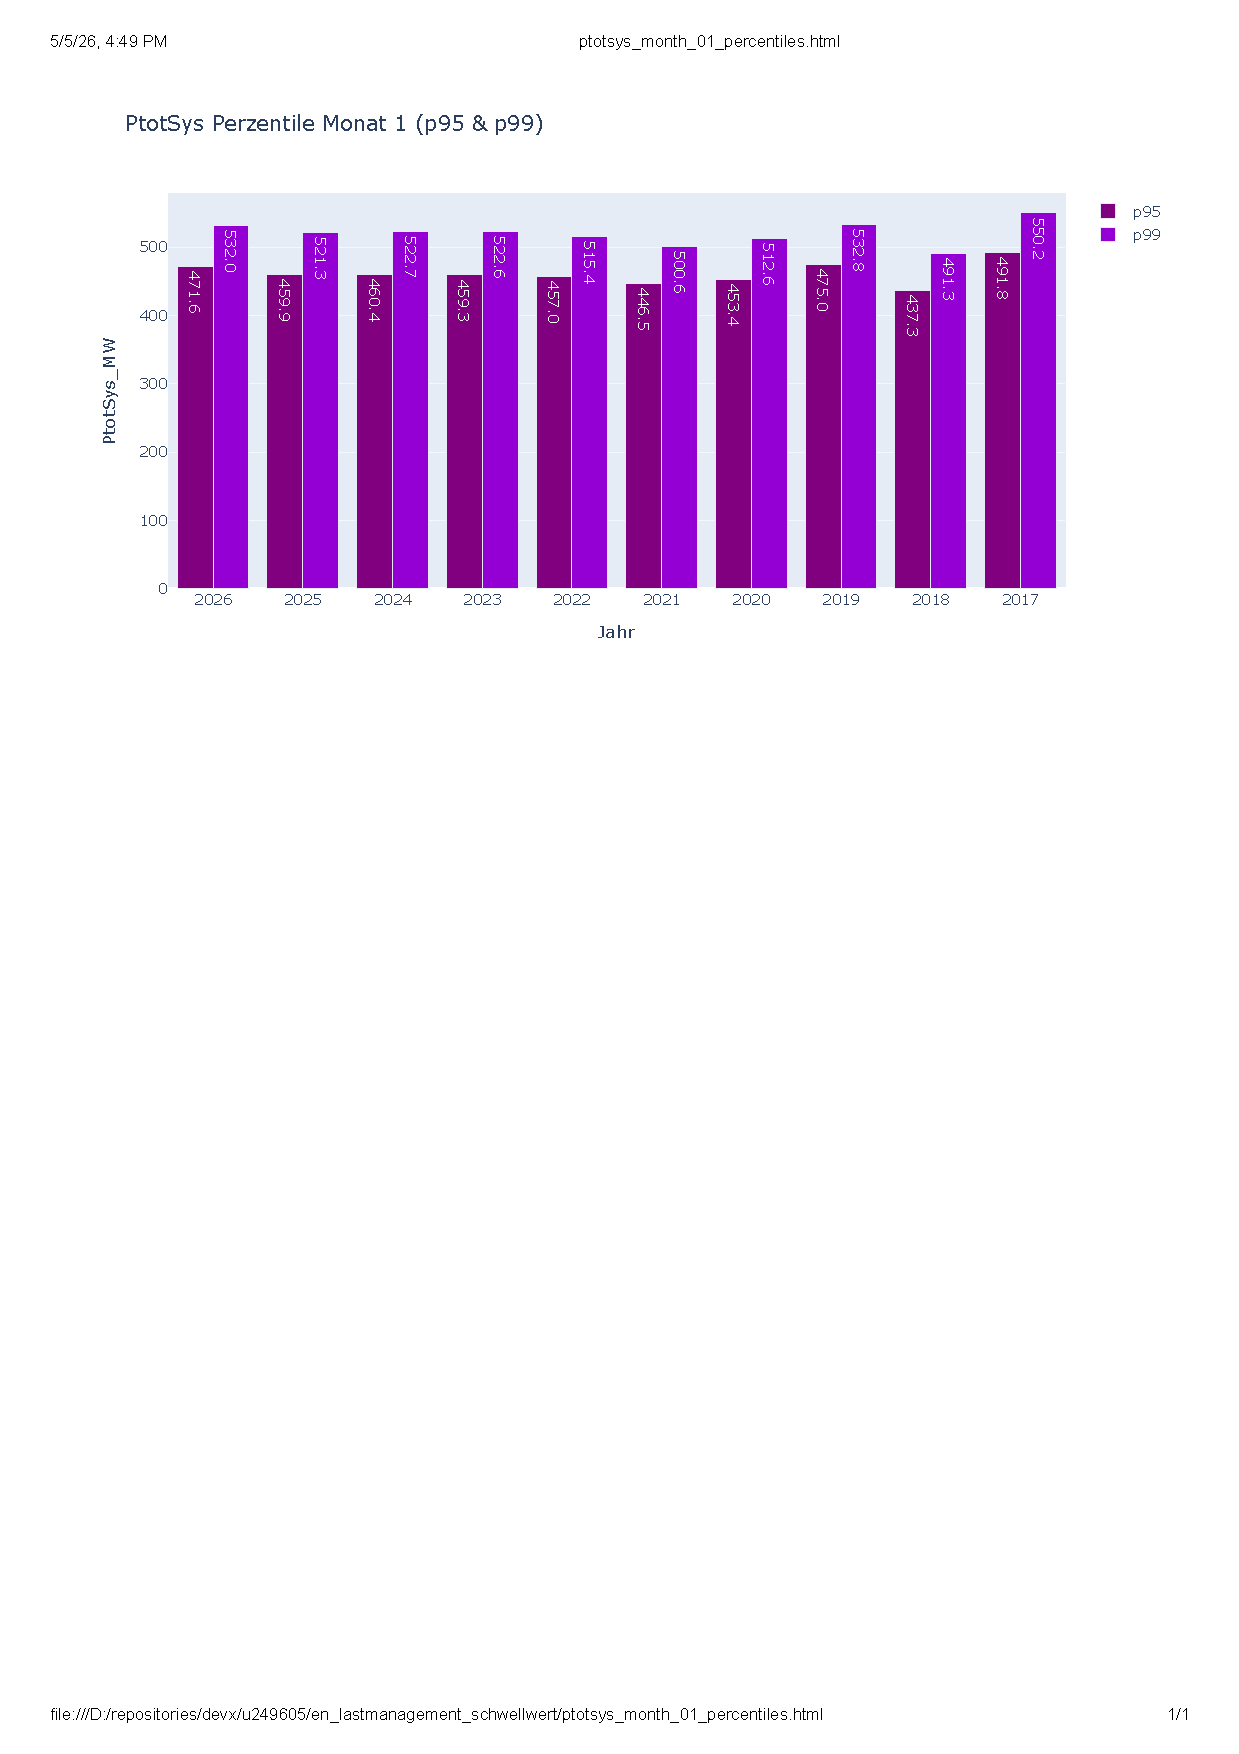
\includegraphics[width=0.95\textwidth,trim={1.2cm 18.6cm 1.2cm 3.1cm},clip]{images/ptotsys_month_01_percentiles.html.pdf}
  \end{center}
\end{frame}

\begin{frame}{Monatswerte Juni (Uebersicht)}
  \textbf{Kennzahlen 2017--2025}
  \vspace{0.3cm}
  \begin{table}[H]
    \centering
    \begin{tabular}{lrrrr}
      \toprule
      Jahr & Mittelwert & Varianz & p95 & p99 \\
      \midrule
      2017 & 269.04 & 9495.50 & 423.49 & 479.27 \\
      2020 & 243.42 & 8427.59 & 388.57 & 441.14 \\
      2021 & 260.29 & 8728.36 & 408.69 & 466.82 \\
      2025 & 260.73 & 10209.47 & 420.17 & 481.63 \\
      \bottomrule
    \end{tabular}
  \end{table}
  \vspace{0.3cm}
  {\small \textbf{Beobachtung:} Deutlicher Rueckgang in 2020 (COVID-19 Effekt)}
\end{frame}

\begin{frame}[fragile]{Juni -- Mittelwerte}
  \begin{center}
    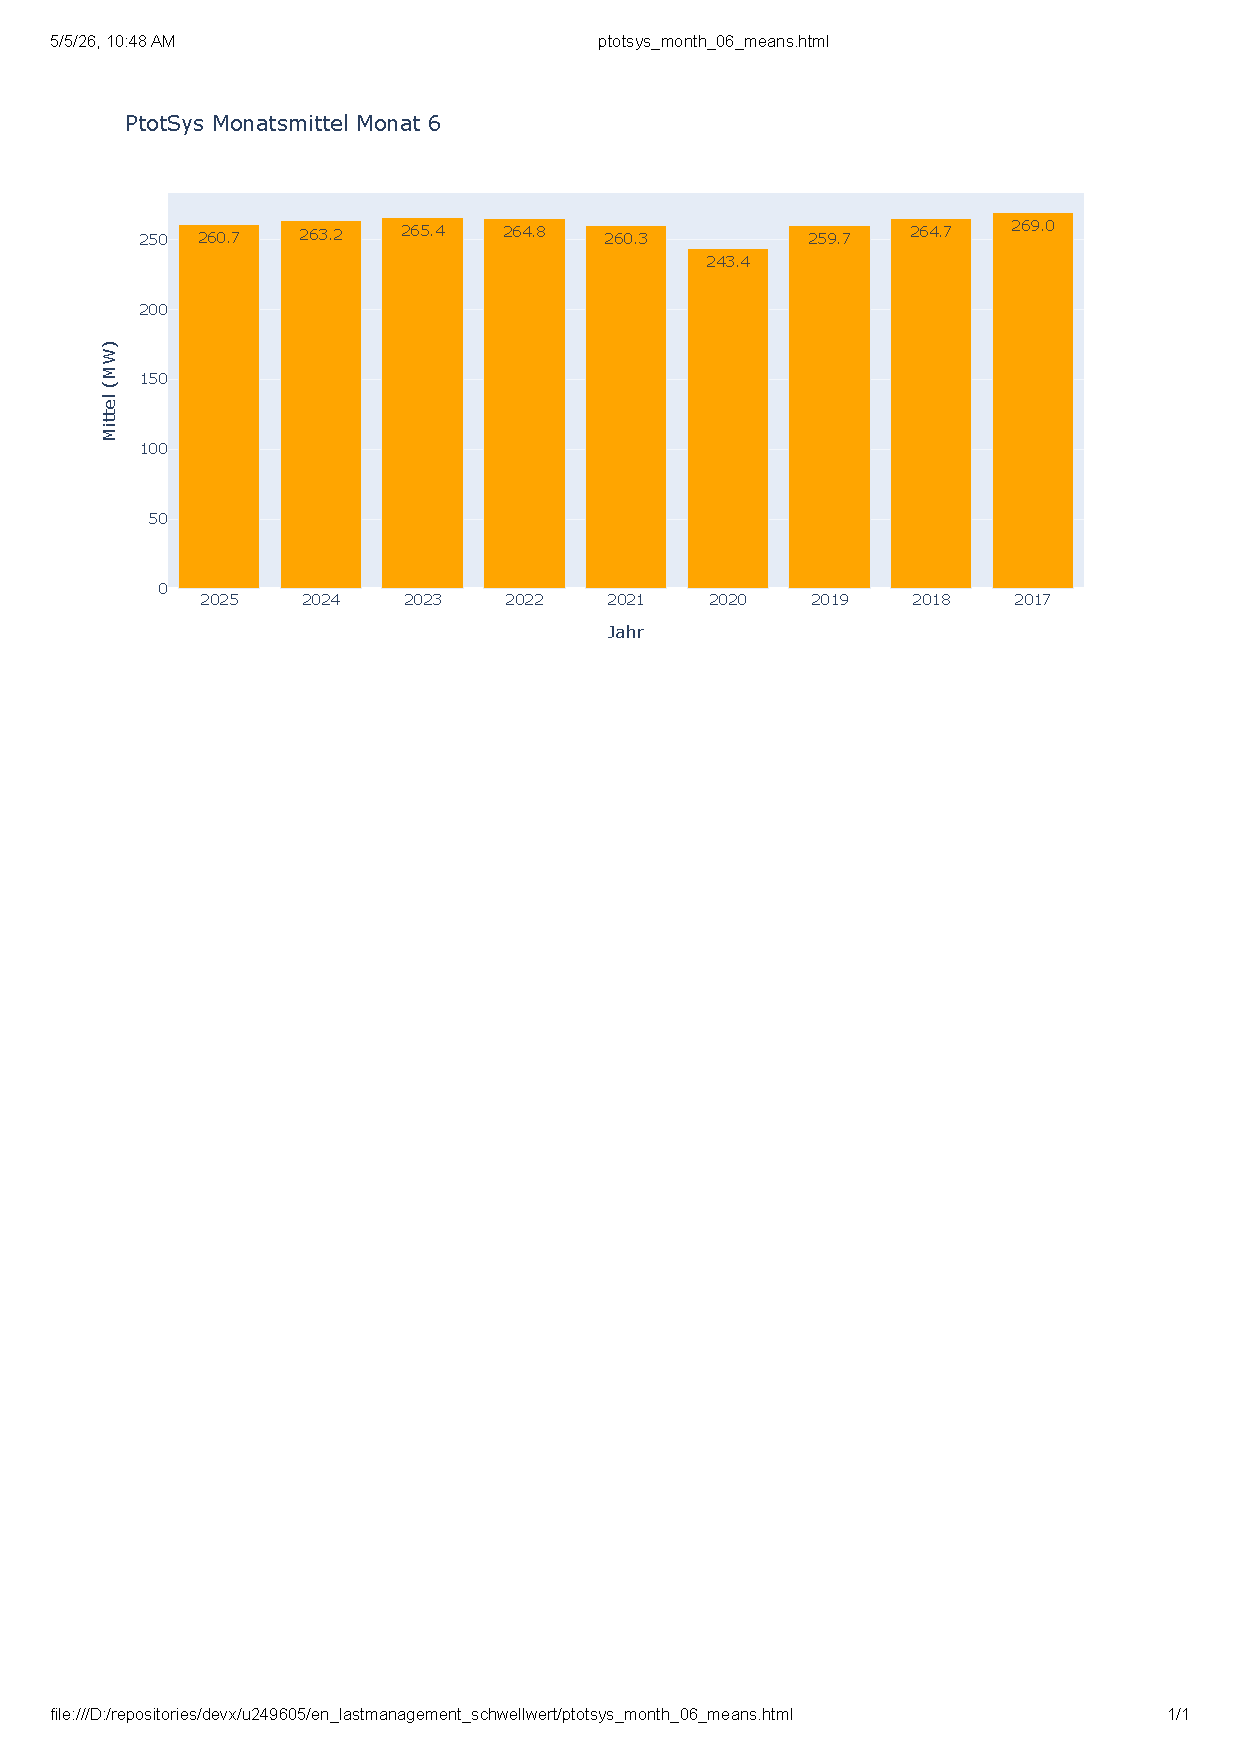
\includegraphics[width=0.95\textwidth,trim={1.2cm 18.9cm 1.2cm 3.1cm},clip]{images/ptotsys_month_06_means.html.pdf}
  \end{center}
\end{frame}

\begin{frame}[fragile]{Juni -- Varianz}
  \begin{center}
    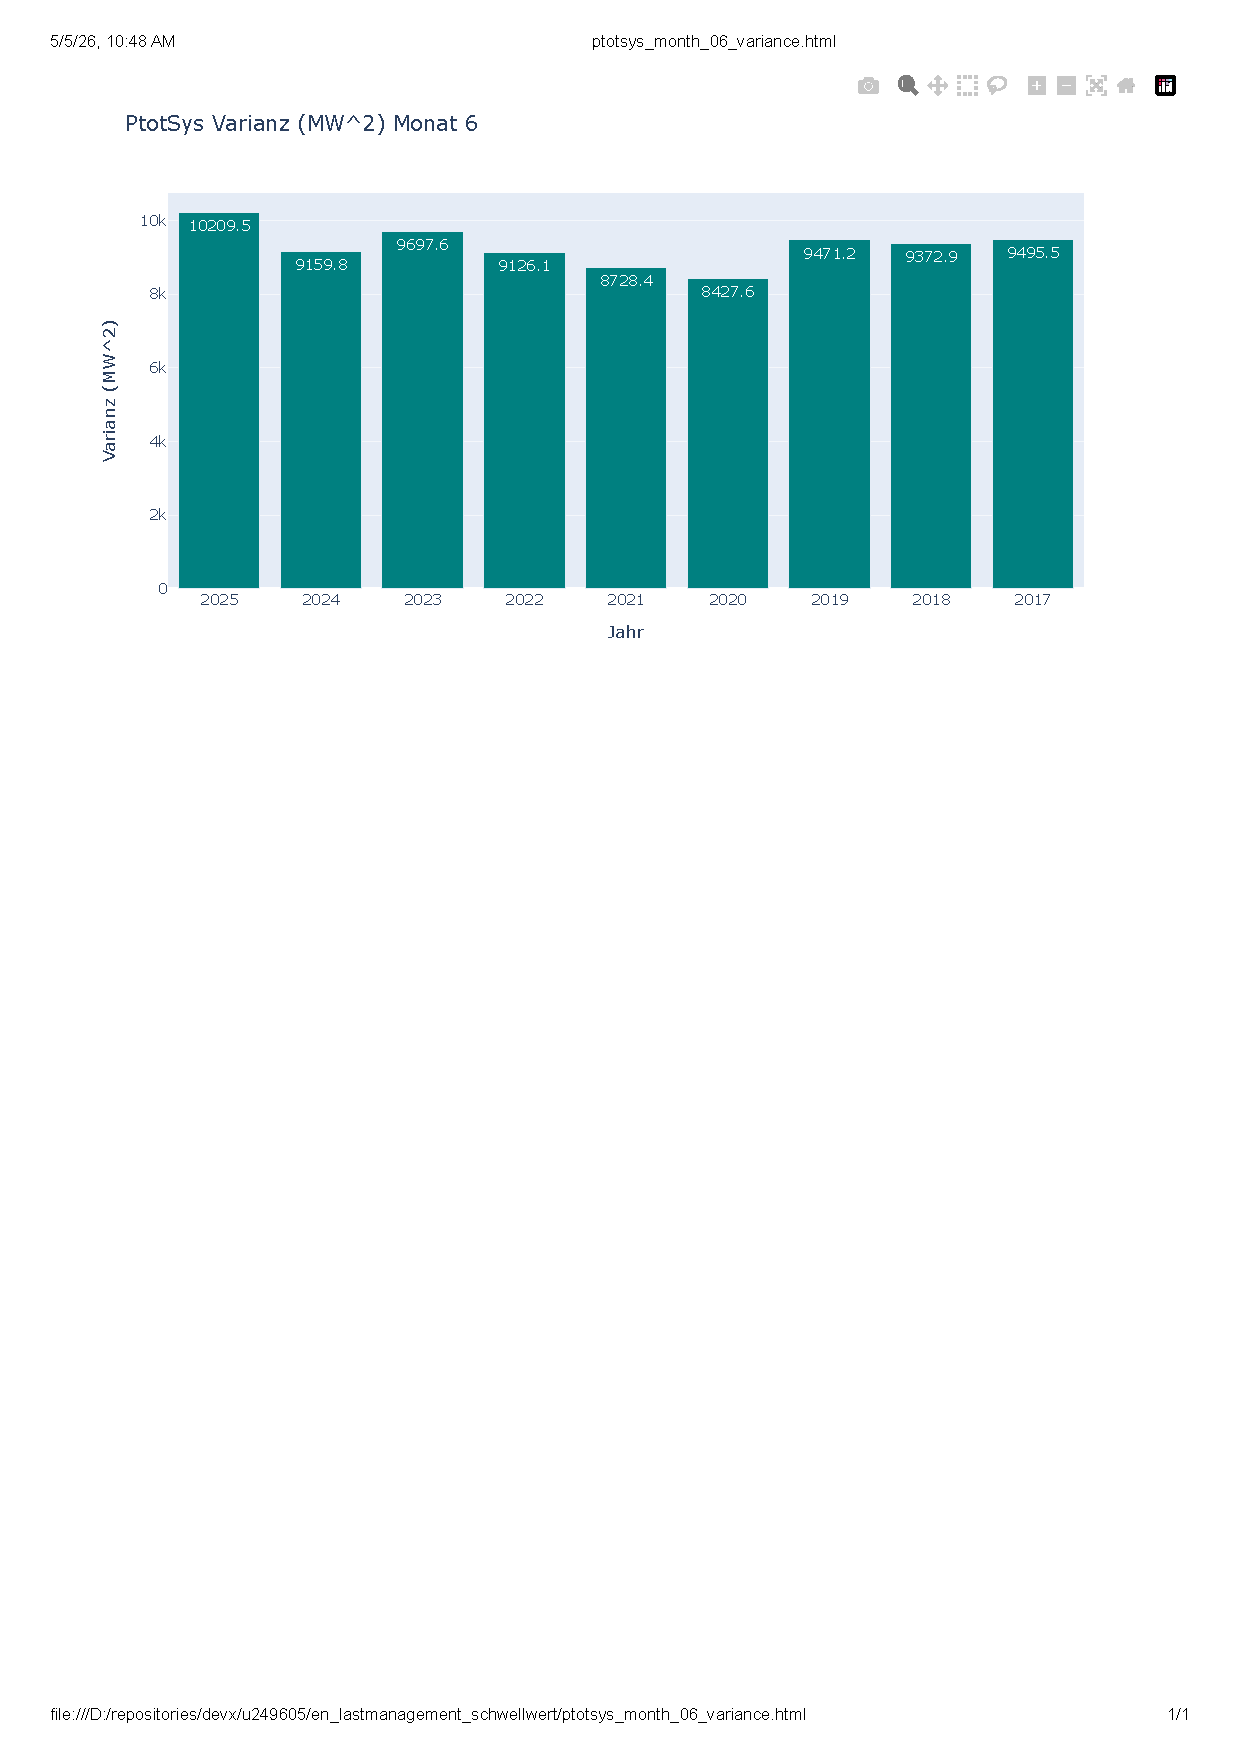
\includegraphics[width=0.95\textwidth,trim={1.2cm 18.6cm 1.2cm 3.1cm},clip]{images/ptotsys_month_06_variance.html.pdf}
  \end{center}
\end{frame}

\begin{frame}[fragile]{Juni -- Perzentile (p95 und p99)}
  \begin{center}
    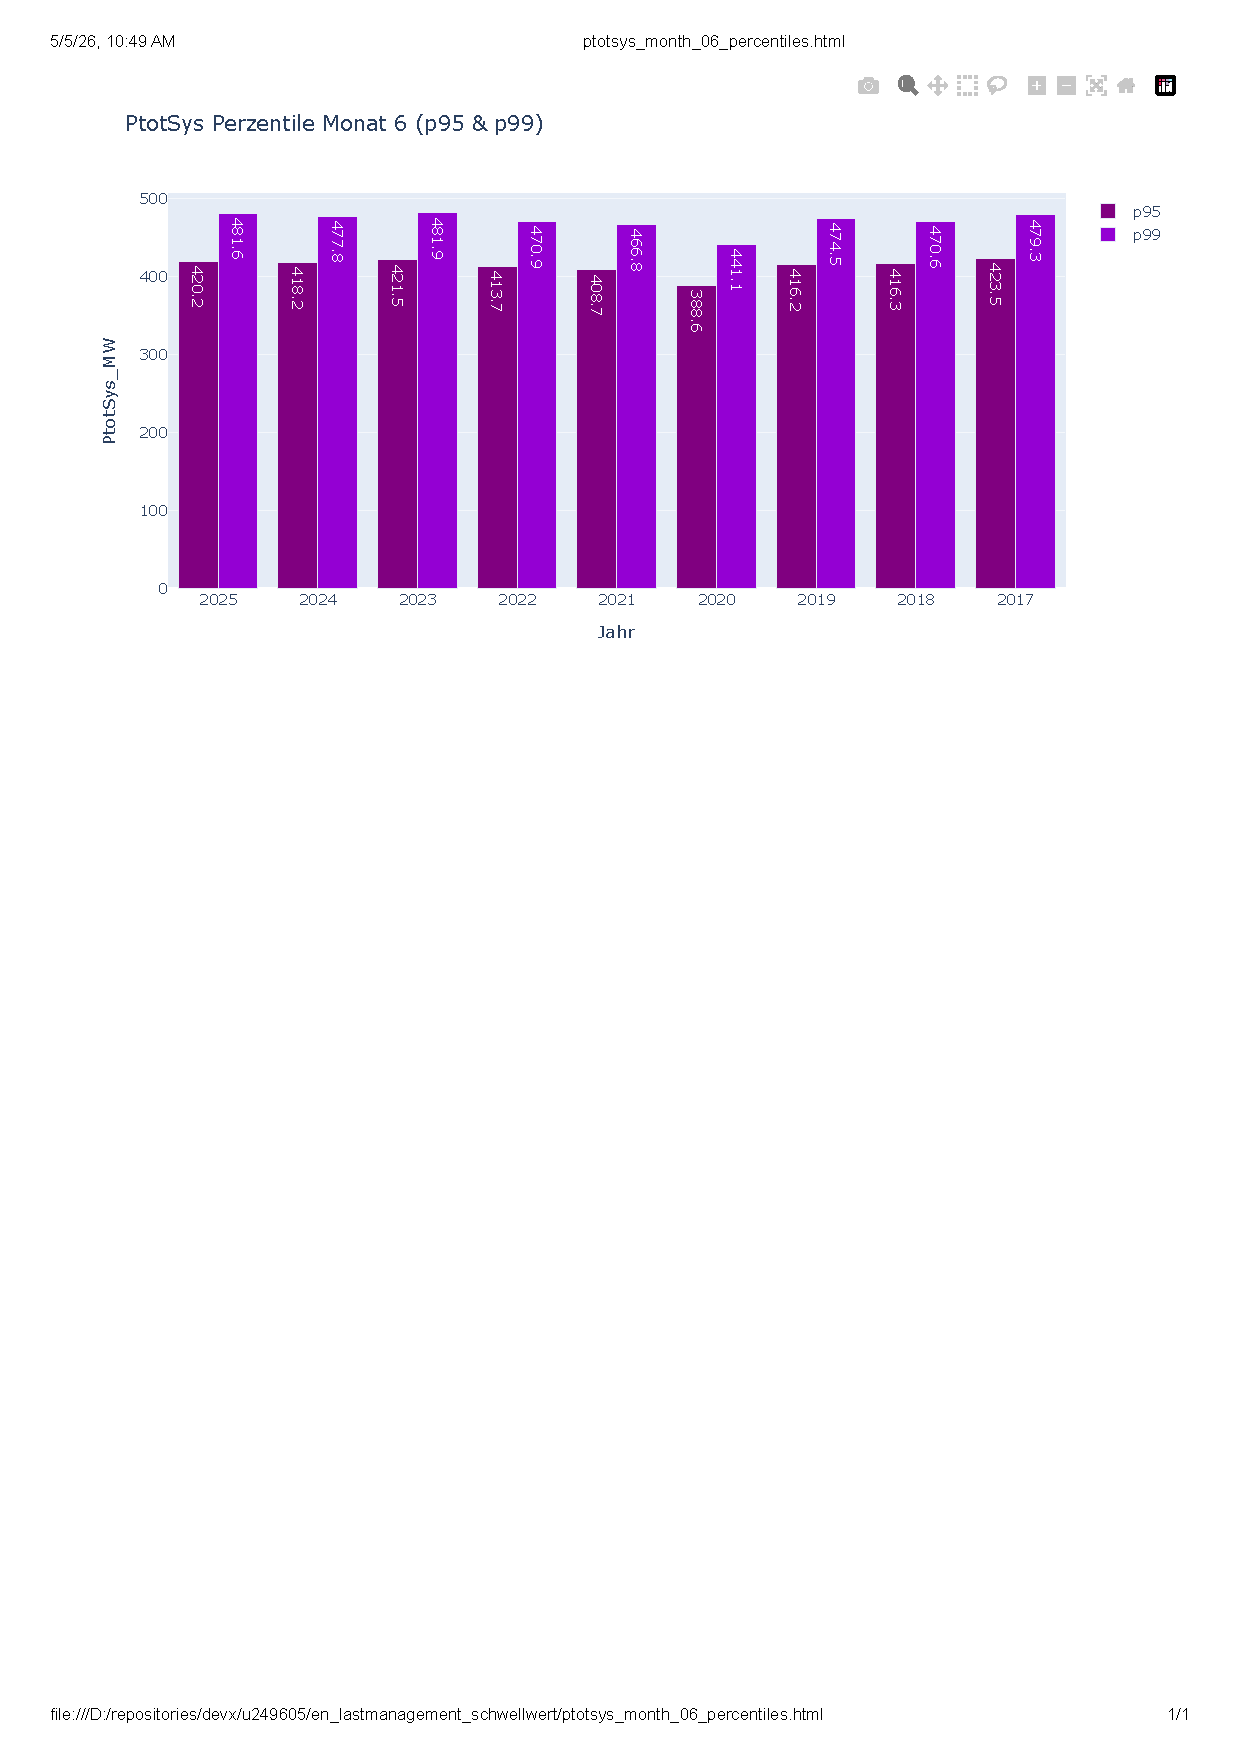
\includegraphics[width=0.95\textwidth,trim={1.2cm 18.6cm 1.2cm 3.1cm},clip]{images/ptotsys_month_06_percentiles.html.pdf}
  \end{center}
\end{frame}

\begin{frame}{Top-3-Peaks pro Jahr als Punktdiagramm}
  \centering
  \begin{tikzpicture}
    \begin{axis}[
      width=0.95\textwidth,
      height=6.8cm,
      xlabel={Jahr},
      ylabel={Ptotsywert [MW]},
      xmin=1996,
      xmax=2025,
      ymin=0,
      ymax=1000,
      xtick={1996,2000,2004,2008,2012,2016,2020,2024},
      scaled x ticks=false,
      xticklabel style={/pgf/number format/fixed,/pgf/number format/precision=0,/pgf/number format/1000 sep={}},
      grid=major,
      legend style={at={(0.5,-0.26)}, anchor=north},
      legend columns=1
    ]
      \addplot+[
        only marks,
        blue,
        mark=diamond*,
        mark options={draw=blue,fill=blue}
      ] coordinates {
        (2014,660.118) (2014,657.526) (2014,655.701)
        (2015,697.533) (2015,671.311) (2015,668.553)
        (2016,714.926) (2016,695.053) (2016,693.241)
        (2017,705.758) (2017,702.726) (2017,690.851)
        (2018,711.028) (2018,706.280) (2018,702.622)
        (2019,745.177) (2019,730.823) (2019,712.230)
        (2020,662.056) (2020,661.553) (2020,659.860)
        (2021,700.802) (2021,680.770) (2021,678.708)
        (2022,761.653) (2022,712.398) (2022,688.306)
        (2023,694.894) (2023,683.628) (2023,679.428)
        (2024,716.878) (2024,712.429) (2024,701.378)
        (2025,736.110) (2025,699.685) (2025,698.890)
      };
      \addlegendentry{Top-3-Peaks (2014--2025)}

      \addplot+[
        only marks,
        green!60!black,
        mark=*,
        mark options={draw=green!60!black,fill=green!60!black}
      ] coordinates {
        (1996,555) (1996,540) (1996,525)
        (1997,560) (1997,545) (1997,530)
        (1998,565) (1998,550) (1998,535)
        (1999,570) (1999,555) (1999,540)
        (2000,590) (2000,575) (2000,560)
        (2001,580) (2001,565) (2001,550)
        (2002,570) (2002,555) (2002,540)
        (2003,600) (2003,585) (2003,570)
        (2004,590) (2004,575) (2004,560)
        (2005,610) (2005,595) (2005,580)
        (2006,670) (2006,650) (2006,630)
        (2007,675) (2007,660) (2007,645)
        (2008,680) (2008,665) (2008,650)
        (2009,690) (2009,675) (2009,660)
        (2010,700) (2010,685) (2010,670)
        (2011,680) (2011,665) (2011,650)
        (2012,720) (2012,705) (2012,690)
      };
      \addlegendentry{Top-3-Peaks Buser (1996--2012)}

      \addplot+[
        only marks,
        red,
        mark=square*,
        mark options={draw=red,fill=red}
      ] coordinates {
        (2000,490) (2000,475) (2000,460)
        (2001,480) (2001,465) (2001,450)
        (2002,470) (2002,455) (2002,440)
        (2003,495) (2003,480) (2003,465)
        (2004,485) (2004,470) (2004,455)
        (2005,505) (2005,490) (2005,475)
        (2006,550) (2006,530) (2006,510)
        (2007,535) (2007,520) (2007,505)
        (2008,545) (2008,530) (2008,515)
        (2009,560) (2009,545) (2009,530)
        (2010,565) (2010,550) (2010,535)
        (2011,545) (2011,530) (2011,515)
        (2012,575) (2012,560) (2012,545)
      };
      \addlegendentry{3 gemessene Top-Viertelstunden im Jahr (2000--2012)}
    \end{axis}
  \end{tikzpicture}
\end{frame}

\begin{frame}[fragile]{Lineare Regression vor der COVID-19-Phase}
  \begin{center}
    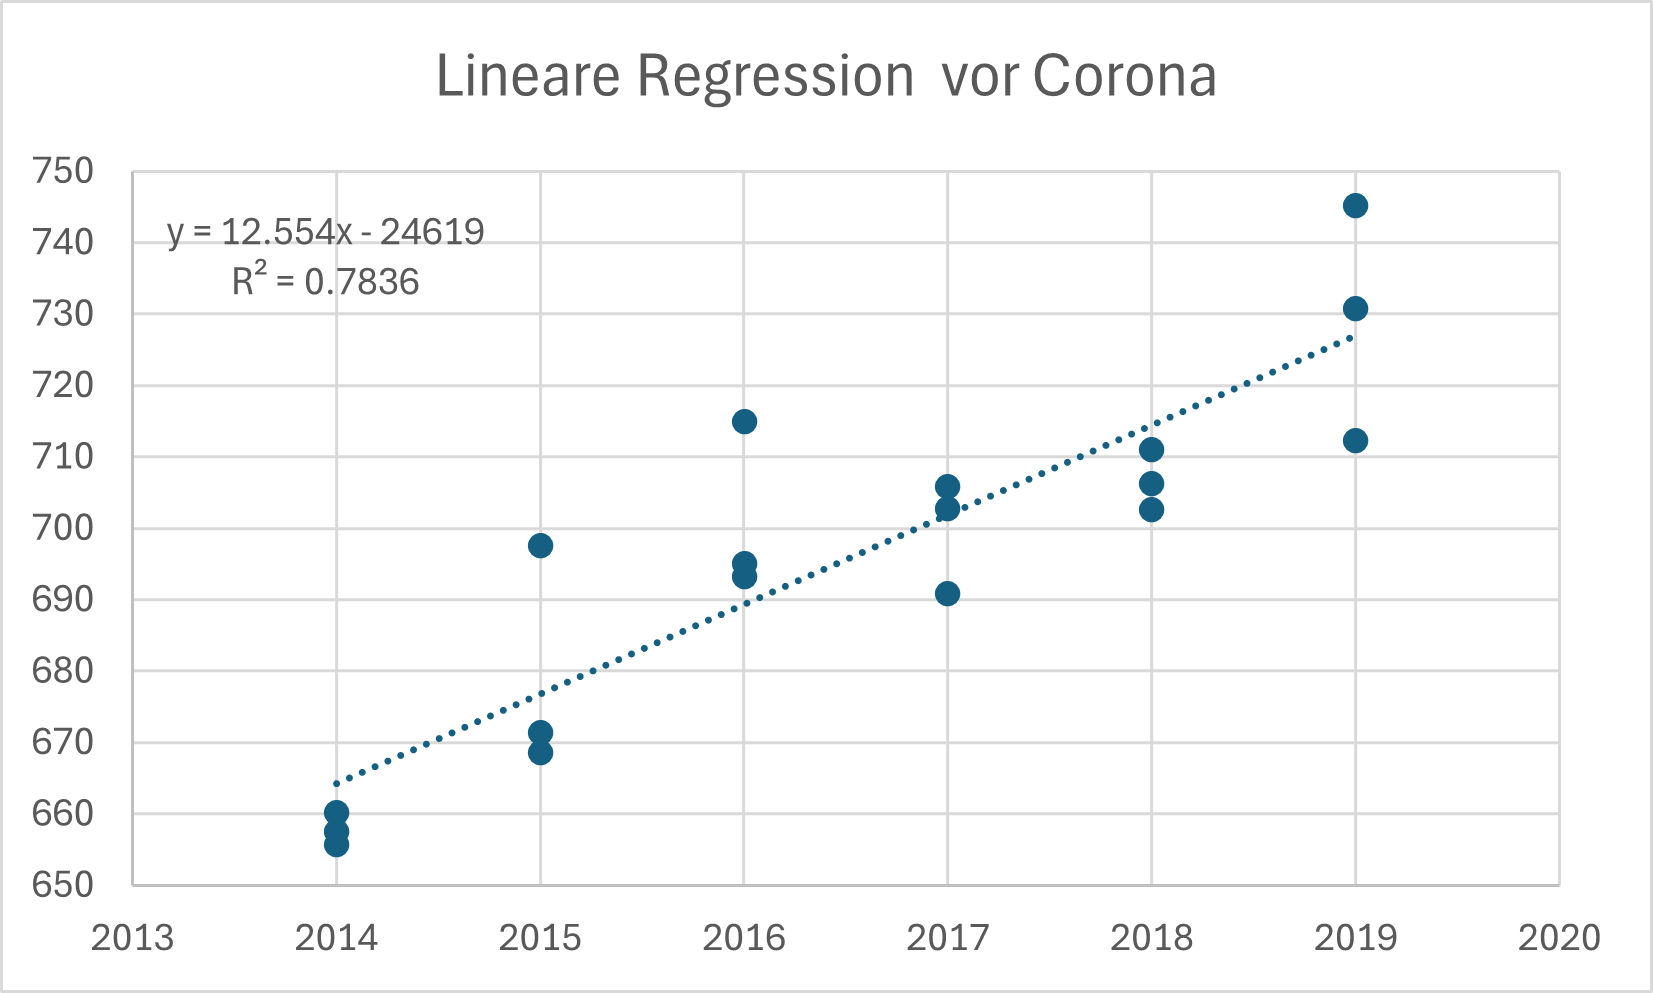
\includegraphics[width=0.92\textwidth]{images/regression/LR_vorCrorna.png}
  \end{center}
\end{frame}

\begin{frame}[fragile]{Lineare Regression waehrend der COVID-19-Phase}
  \begin{center}
    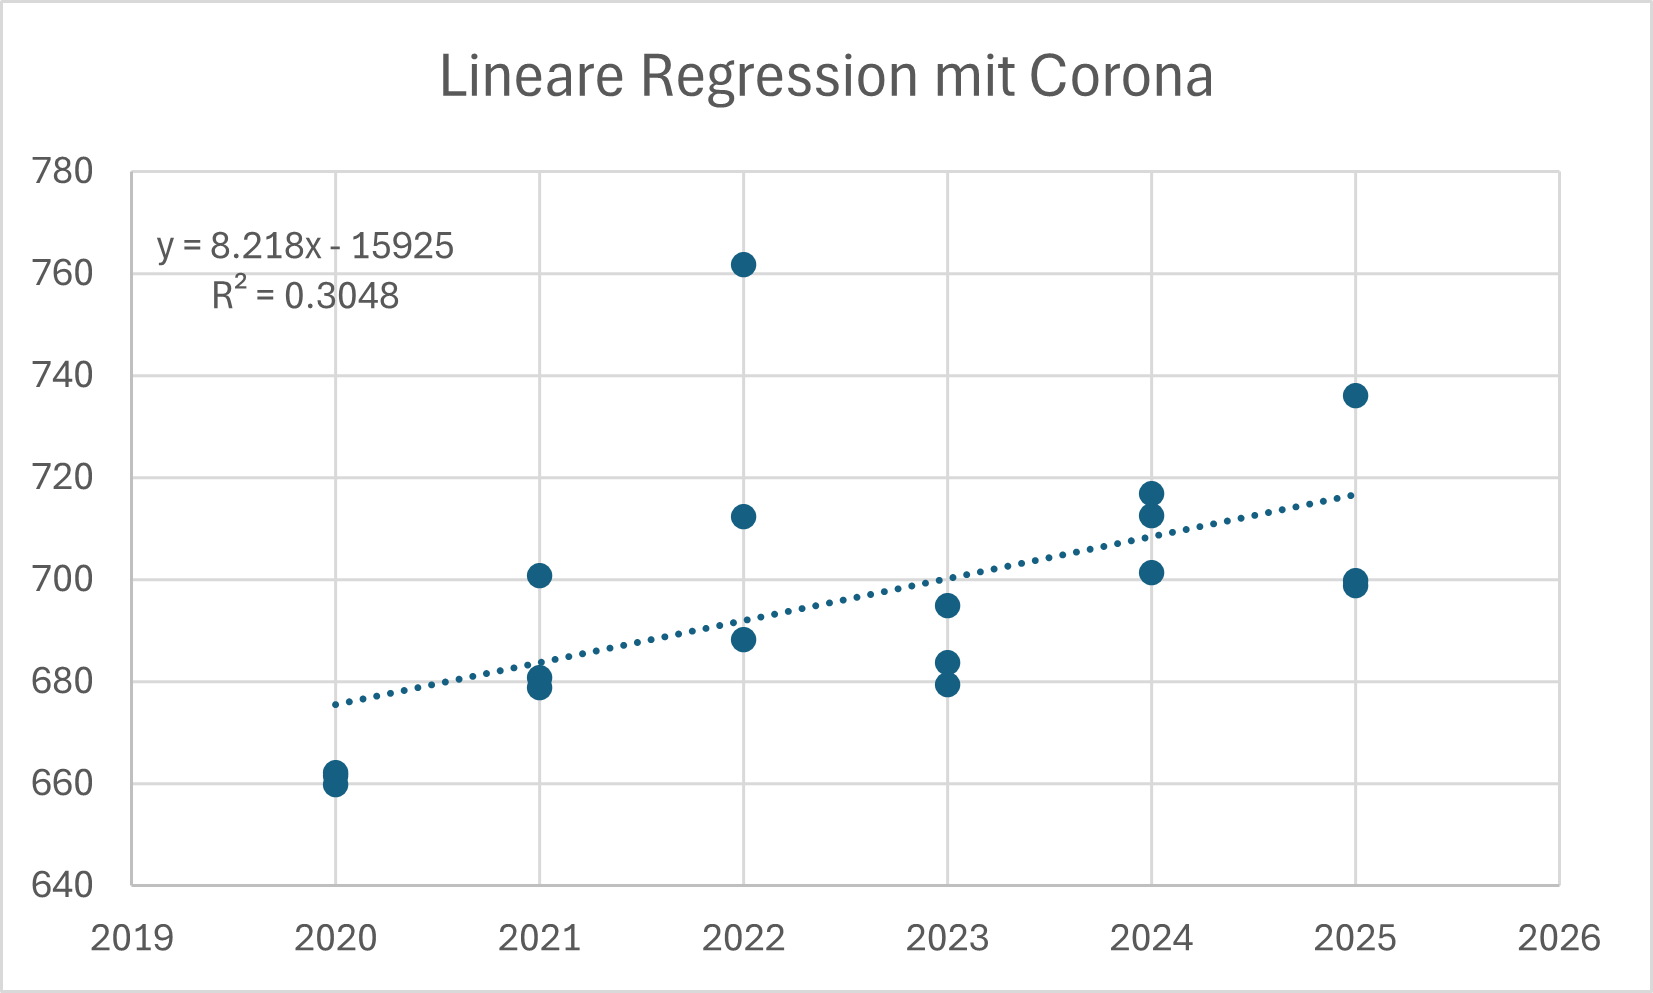
\includegraphics[width=0.92\textwidth]{images/regression/LR_mitCorona.png}
  \end{center}
\end{frame}

\begin{frame}[fragile]{Lineare Regression nach der COVID-19-Phase}
  \begin{center}
    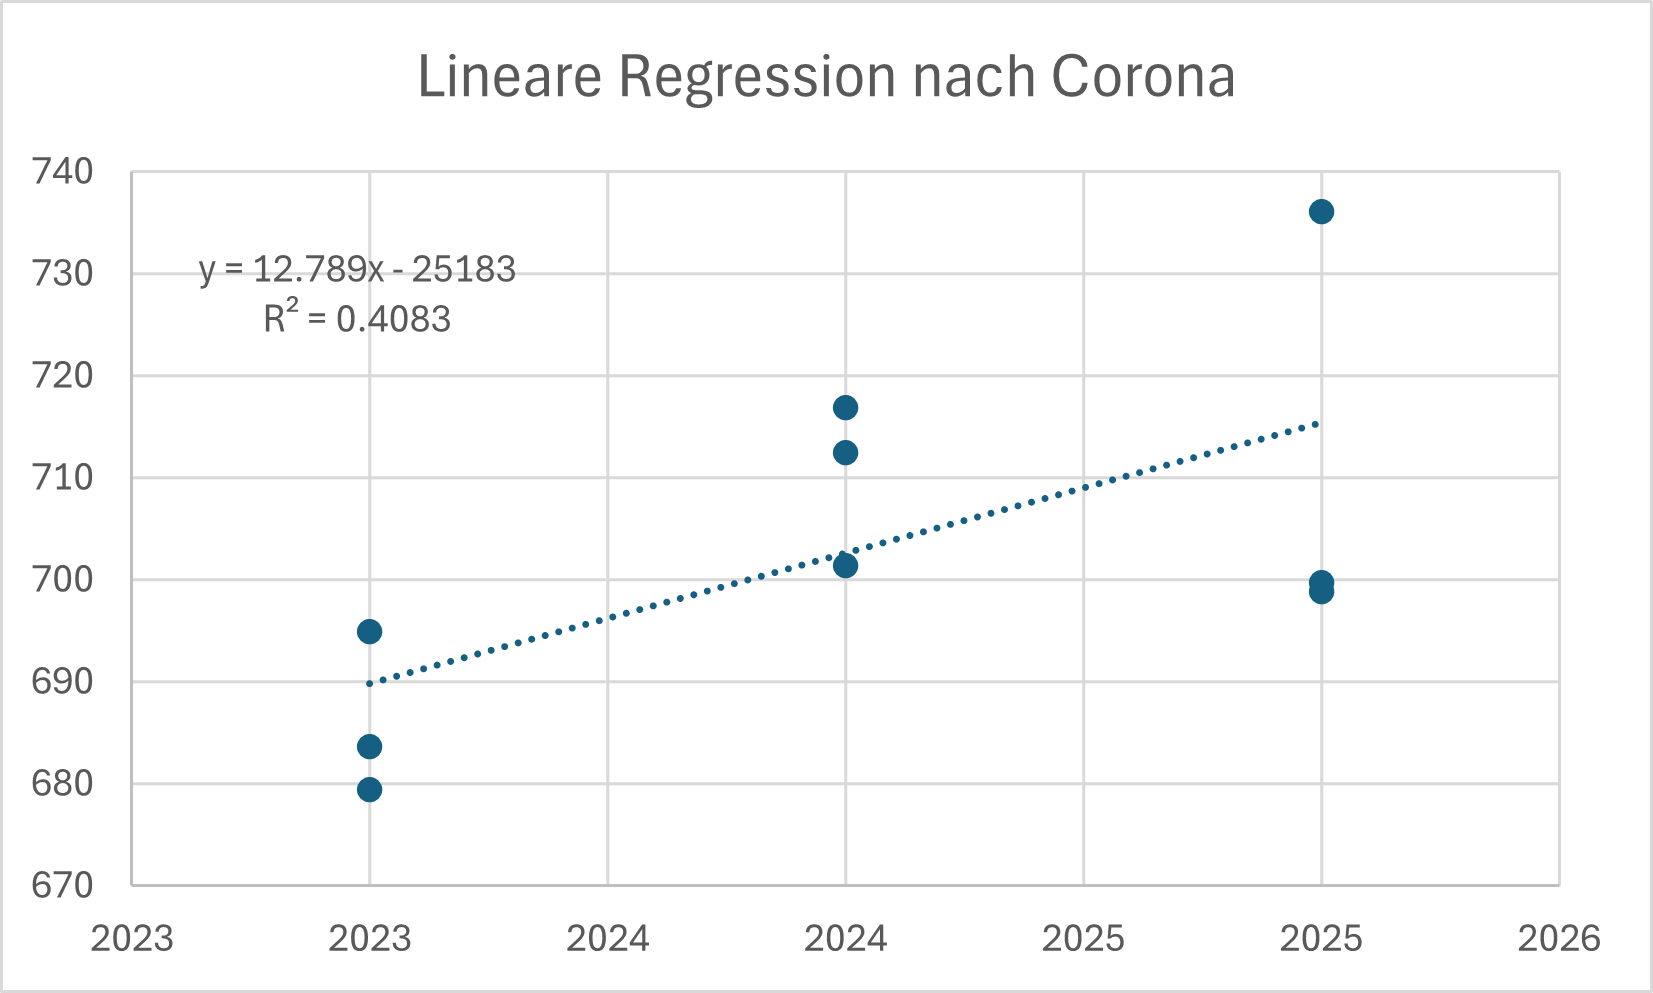
\includegraphics[width=0.92\textwidth]{images/regression/LR_nachCorona.png}
  \end{center}
\end{frame}

\begin{frame}{FFT-Vergleich Januar bis Februar}
  \begin{columns}[T]
    \column{0.56\textwidth}
    \textbf{Kernaussagen:}
    \begin{itemize}
      \item Vergleich der Jahre 2016, 2019, 2021, 2023 und 2025
      \item Mittelwert der Amplitude ueber alle $k=1\dots86400$
      \item 2016 weist das hoechste Gesamtniveau auf
      \item 2025 liegt ueber 2019, 2021 und 2023, aber unter 2016
      \item Groesste Unterschiede bei kleinen harmonischen Ordnungen
    \end{itemize}

    \column{0.44\textwidth}
    \begin{table}[H]
      \scriptsize
      \centering
      \begin{tabular}{lr}
        \toprule
        Jahr & Mittelwert \\
        \midrule
        2016 & 0.179231 \\
        2019 & 0.148302 \\
        2021 & 0.147947 \\
        2023 & 0.148525 \\
        2025 & 0.155847 \\
        \bottomrule
      \end{tabular}
    \end{table}
    \vspace{0.2cm}
    {\scriptsize
    \textbf{Differenzen:}\\
    $\Delta_{23-16}=-0.030706$\\
    $\Delta_{25-16}=-0.023384$\\
    $\Delta_{25-23}=0.007322$}
  \end{columns}
\end{frame}

\begin{frame}[fragile]{FFT Januar bis Februar -- Balkendiagramm}
  \begin{center}
    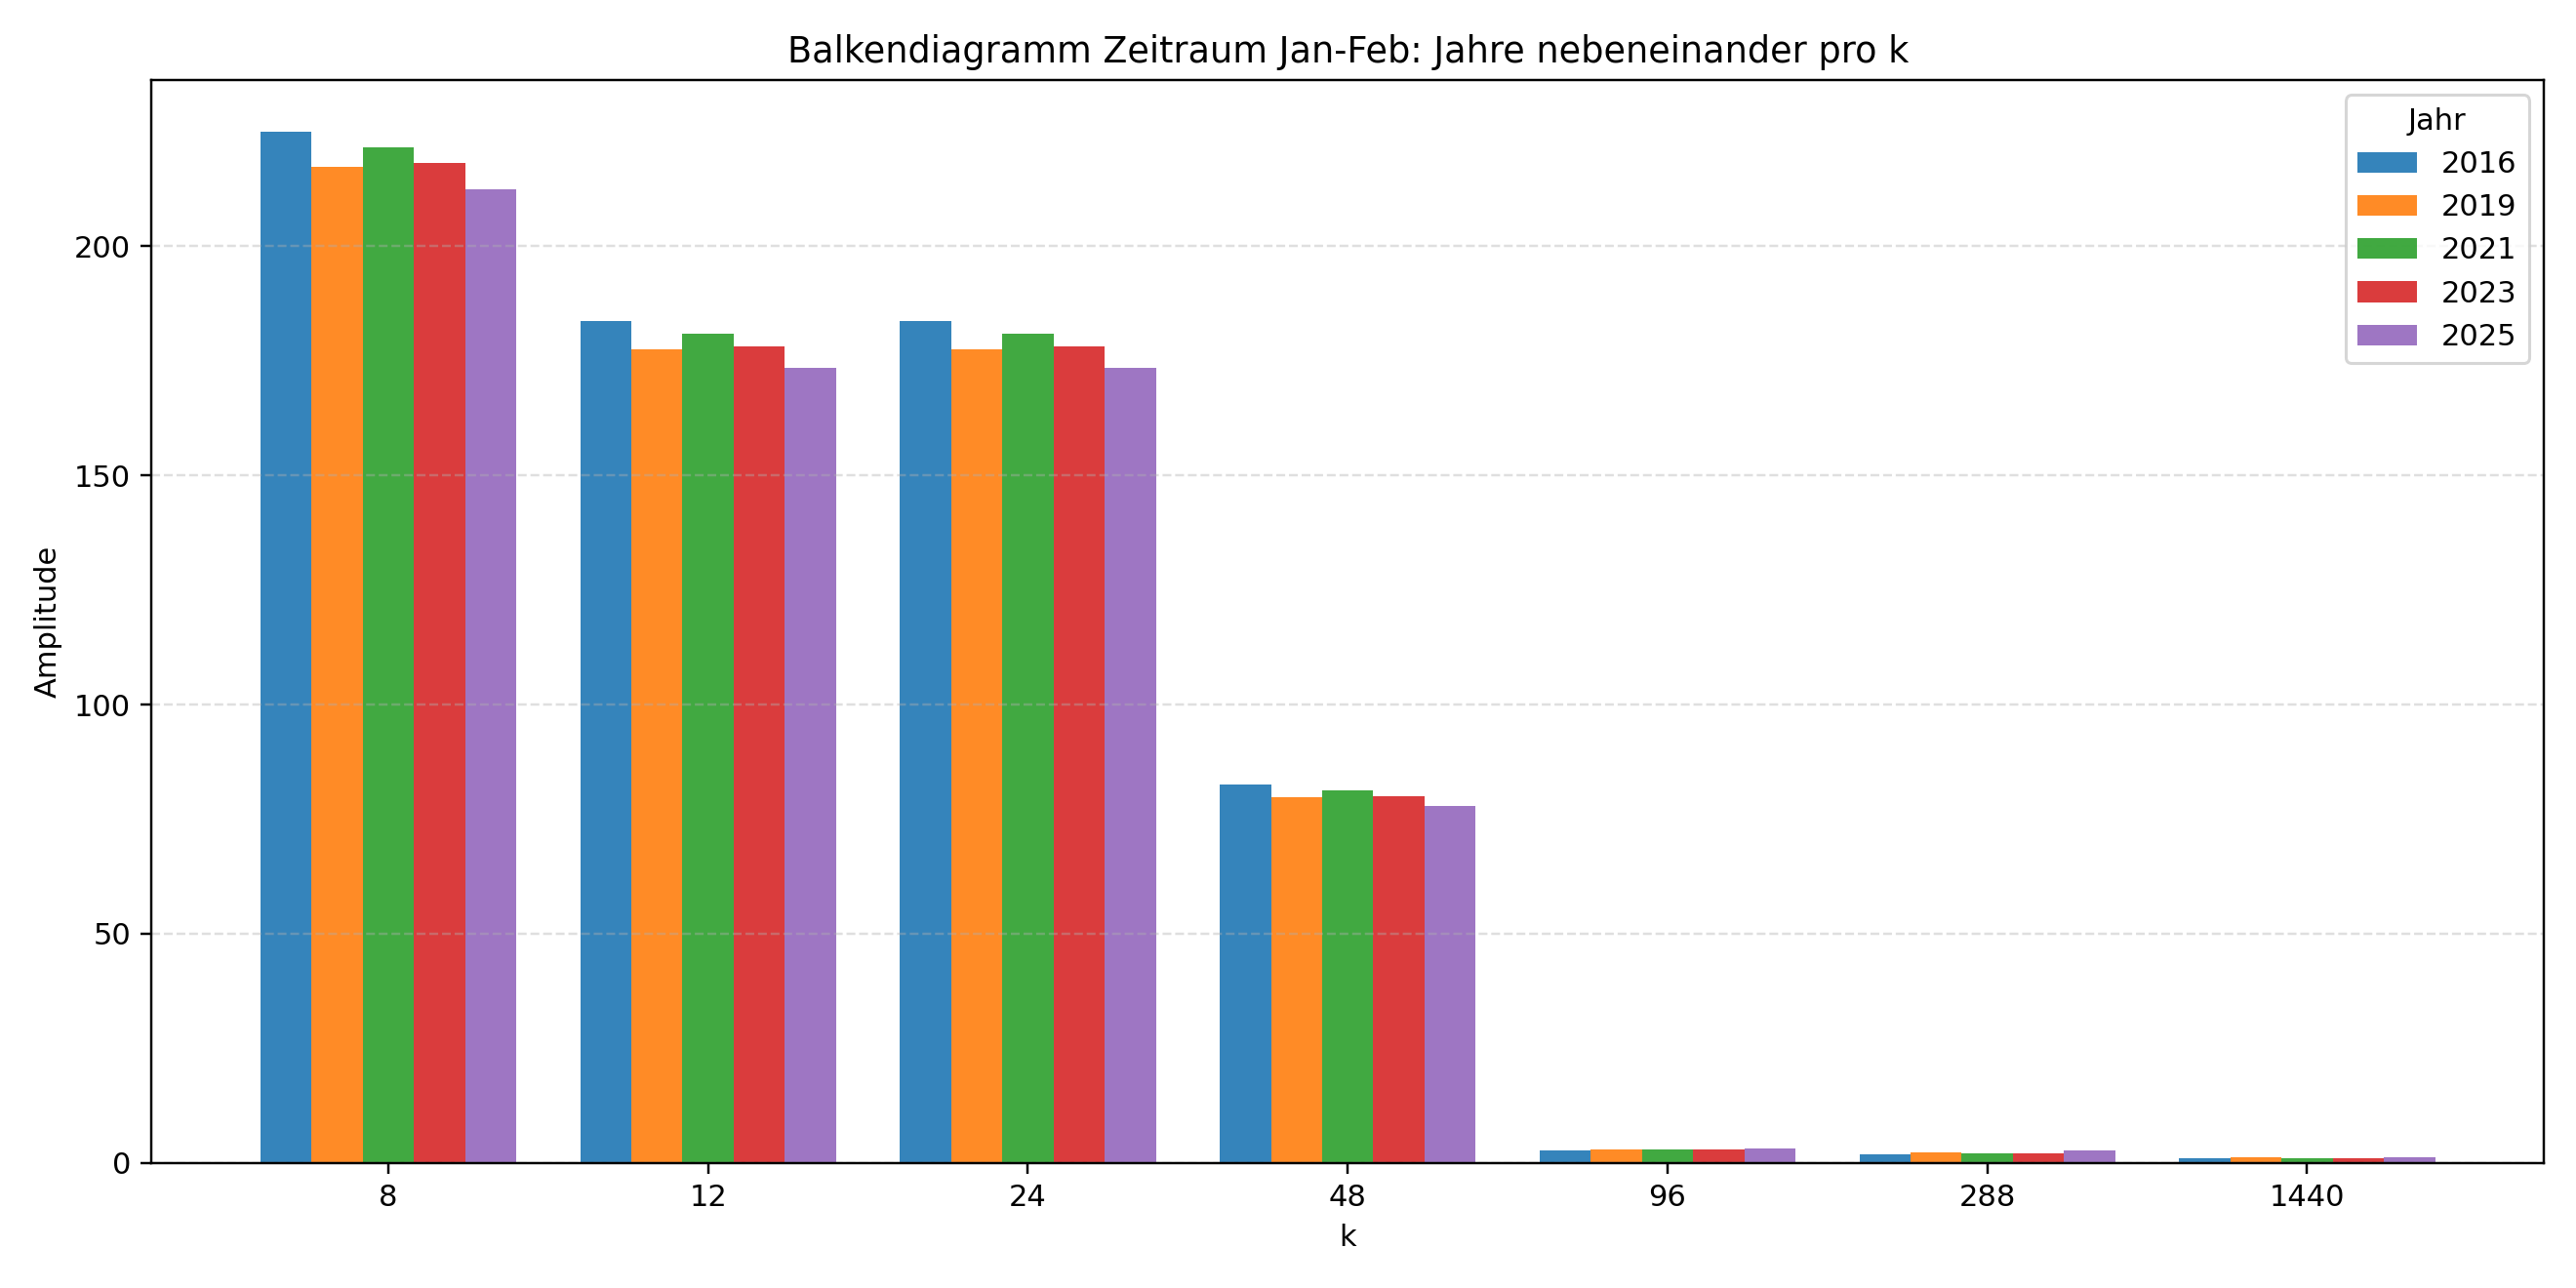
\includegraphics[width=0.92\textwidth]{images/k_barplots_by_year/k_barplot_grouped_years_kwfrom.png}
  \end{center}
\end{frame}

\begin{frame}{FFT-Vergleich Juni bis August}
  \begin{columns}[T]
    \column{0.56\textwidth}
    \textbf{Kernaussagen:}
    \begin{itemize}
      \item Sommerzeitraum zeigt ein deutlich stabileres Bild
      \item 2016, 2021 und 2023 liegen sehr nahe beieinander
      \item 2025 weist den hoechsten Mittelwert auf
      \item 2019 liegt im Mittel unter den uebrigen Jahren
      \item Unterschiede konzentrieren sich erneut auf kleine $k$
    \end{itemize}

    \column{0.44\textwidth}
    \begin{table}[H]
      \scriptsize
      \centering
      \begin{tabular}{lr}
        \toprule
        Jahr & Mittelwert \\
        \midrule
        2016 & 0.138100 \\
        2019 & 0.130053 \\
        2021 & 0.138413 \\
        2023 & 0.137598 \\
        2025 & 0.143206 \\
        \bottomrule
      \end{tabular}
    \end{table}
    \vspace{0.2cm}
    {\scriptsize
    \textbf{Differenzen:}\\
    $\Delta_{23-16}=-0.000502$\\
    $\Delta_{25-16}=0.005106$\\
    $\Delta_{25-23}=0.005608$}
  \end{columns}
\end{frame}

\begin{frame}[fragile]{FFT Juni bis August -- Balkendiagramm}
  \begin{center}
    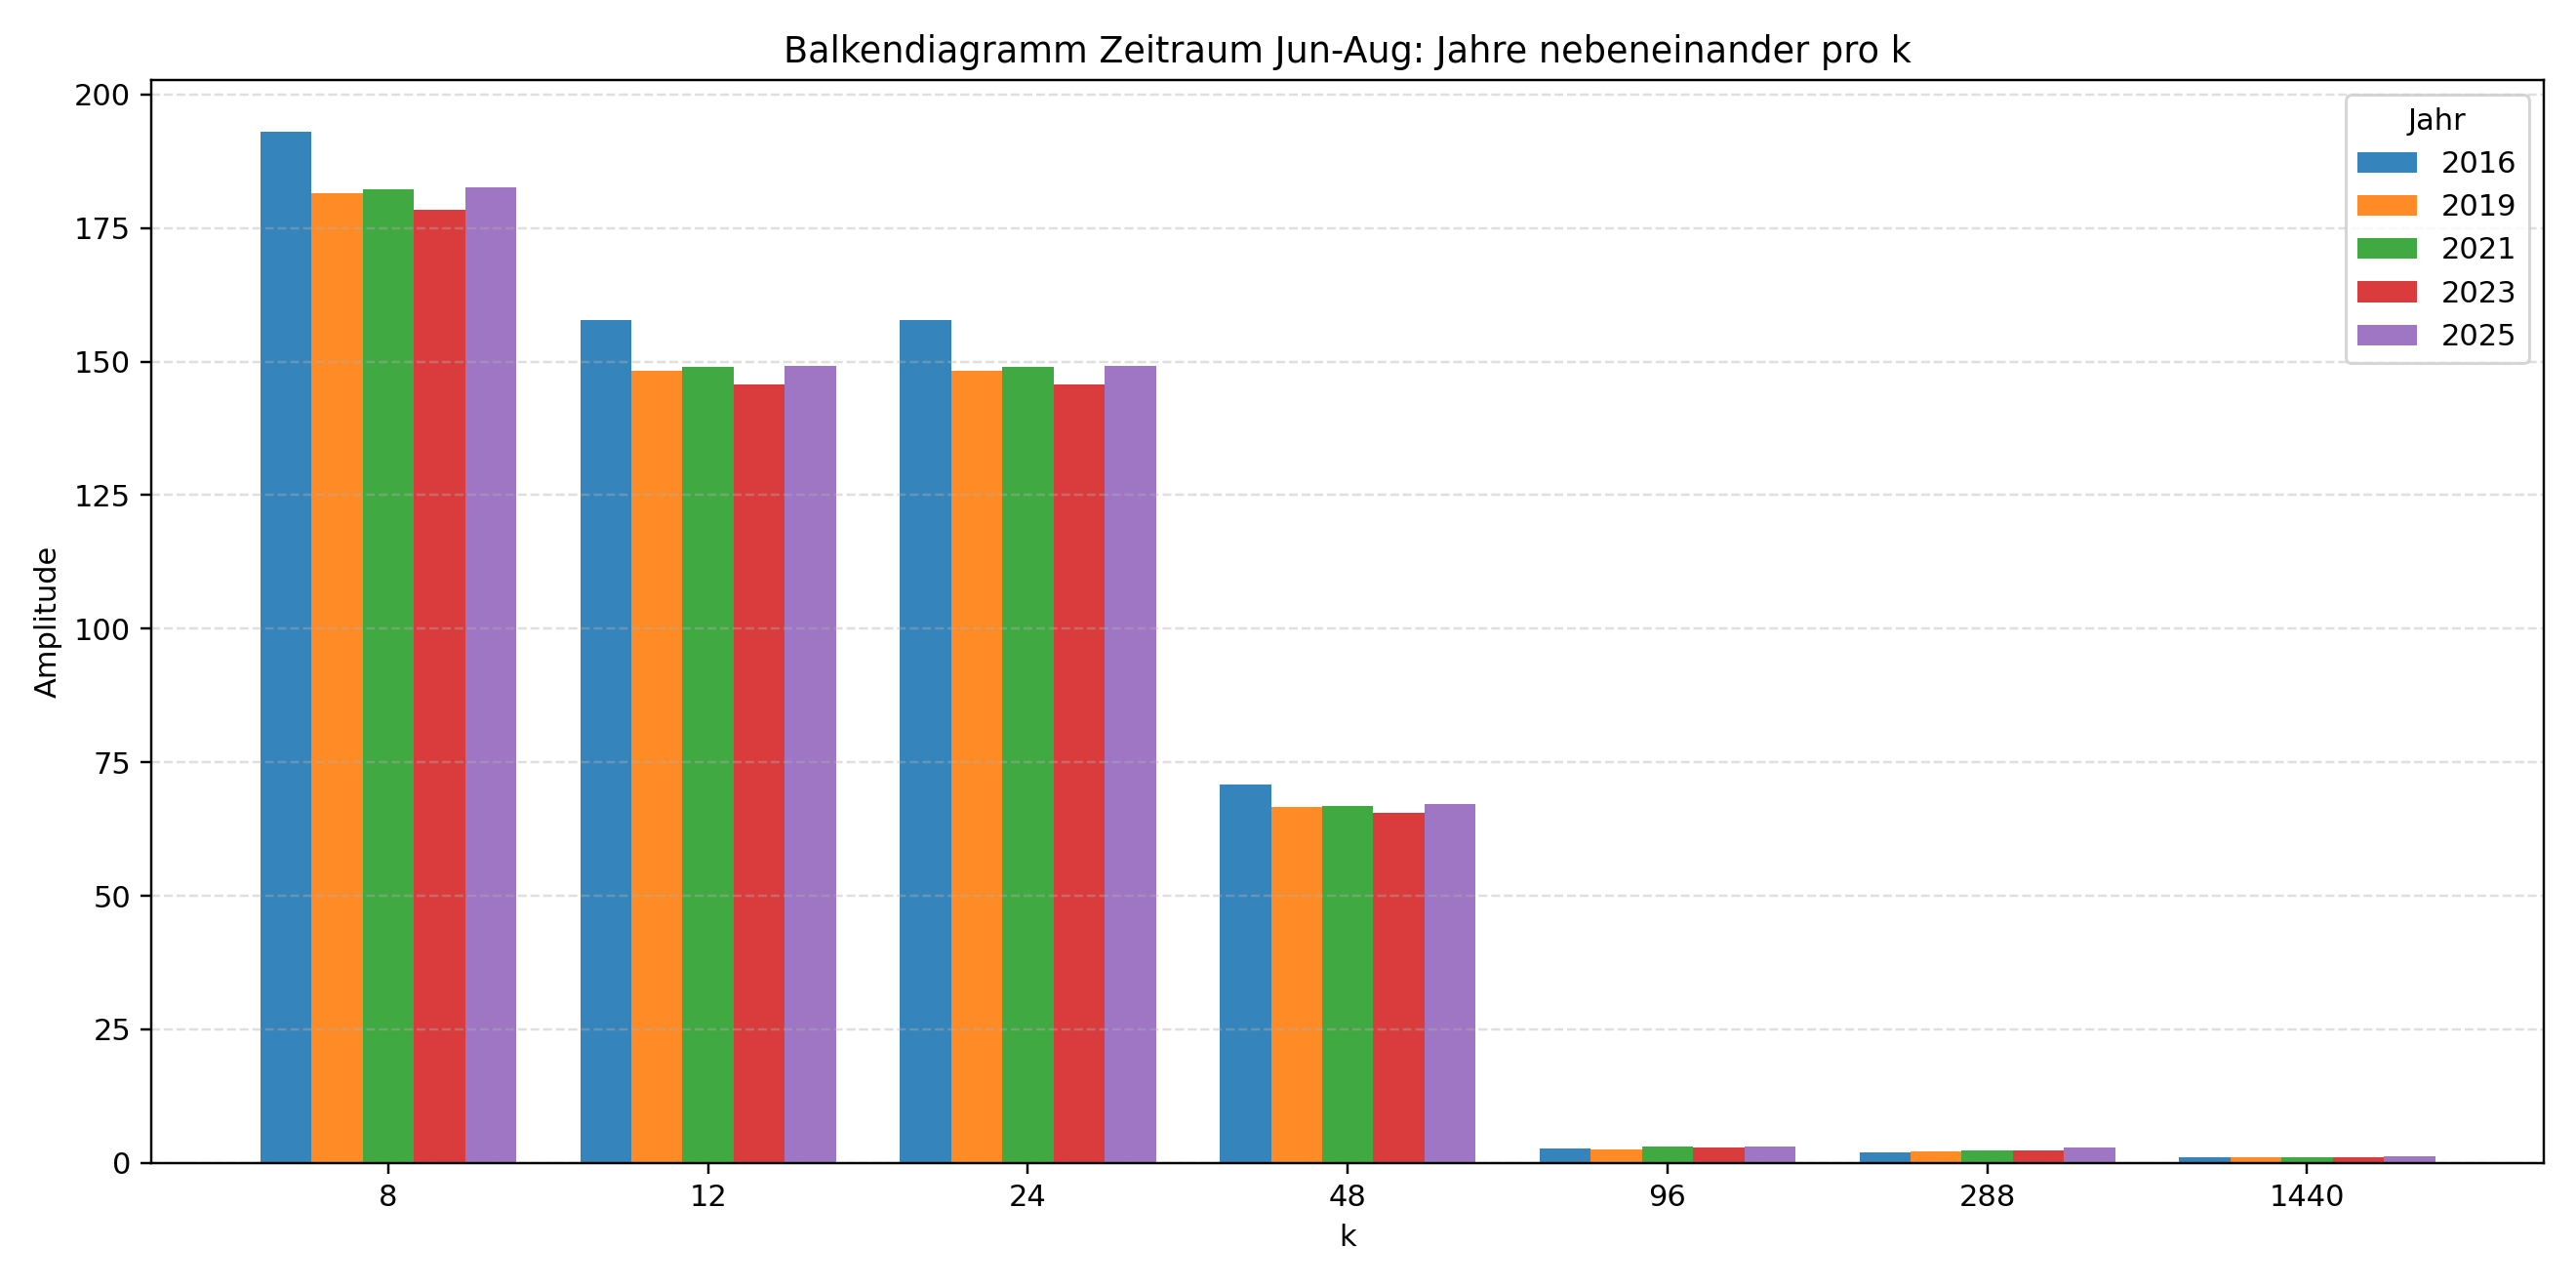
\includegraphics[width=0.92\textwidth]{images/k_barplots_by_year/k_barplot_grouped_years_kwfrom_jun_aug.png}
  \end{center}
\end{frame}

\begin{frame}{Diskussionspunkte}
  \begin{itemize}
    \setlength{\itemsep}{0.7em}
    \item Meteo-Daten
    \item Pünktlichkeit
    \item Lastmanagement
    \item Installierte Leistung
    \item Personenkilometer
    \item Tonnenkilometer
  \end{itemize}
\end{frame}

\begin{frame}[plain]
  \vfill
  \begin{center}
    \huge\textbf{\color{sbbred}{\rmfamily Vielen Dank!}}
  \end{center}
  \vfill
\end{frame}

\end{document}
